\documentclass{beamer}
\usepackage{graphicx}

\usetheme{Execushares}

\def\imgpostfix{-small}

\begin{document}
\title{Design Review: MorphCore}
\subtitle{Amanda Marano, Brian Jacobs, Pete Ehrett}
\author{Team DRRA}
\date{\today}

\frame{\titlepage}

\frame{
  \tableofcontents
}

\section{System Overview}
\frame{
  \frametitle{System Overview}
  \begin{center}
    \begin{tabular}{c c}
      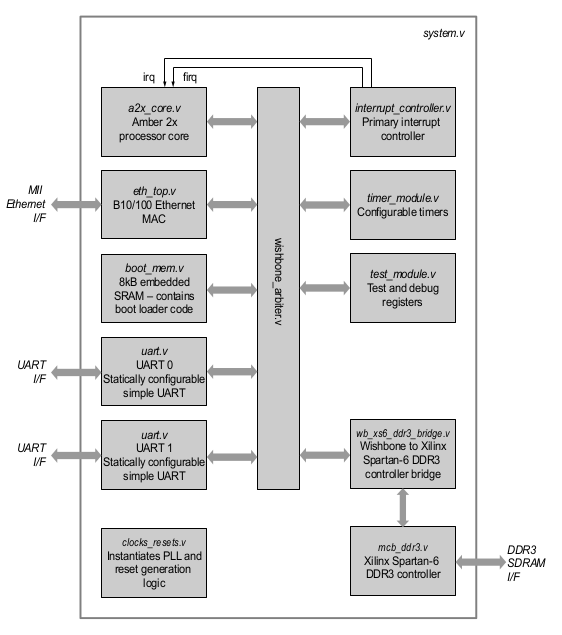
\includegraphics[height=2.5in]{Diagrams/System-Diagram.png} &
      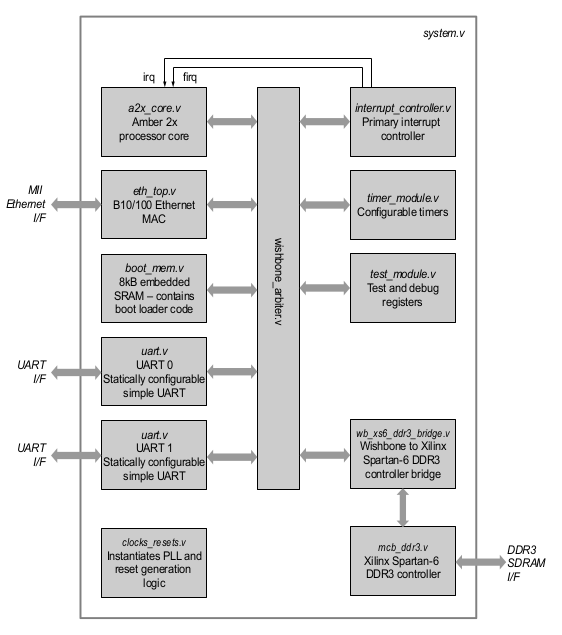
\includegraphics[height=2.5in]{Diagrams/System-Diagram.png}\\
      \textit{Amber System} & \textit{Our System} \\
    \end{tabular}
  \end{center}
}

\frame{
  \frametitle{System Overview}
  \begin{itemize}
    \item Existing system
      \begin{itemize}
        \item DDR3 memory
        \item Ethernet, UART
        \item Interrupt controller
        \item Amber 25 Core
      \end{itemize}
    \item Our changes
    \begin{itemize}
      \item We are ignoring Ethernet
      \item UART lets us program the core
      \item Adding HDMI and PS/2 user interface components
      \item Replacing Amber 25 with our modified core
    \end{itemize}
  \end{itemize}
}

\section{Amber Core Architectural Overview}
\frame{
  \frametitle{Amber Core Architecture}
  \begin{itemize}
    \item Our starting point is the Amber 25 core.
    \item 5 stage pipeline: Fetch, Decode, Execute, Memory, Writeback
    \item Based on the ARMv7 ISA
    \item No thumb instructions
    \item Targetable with gcc cross compilation
  \end{itemize}
  \vspace{.25in}
  \colorbox{black}{
    \begin{minipage}{3.99in}
      \tiny\texttt{\textcolor{green}{DRRA@fuggle\$} \textcolor{white}{arm-xilinx-linux-gnueabi-gcc -c -march=armv2a -mno-thumb-interwork -I../../sw/include -o program.o program}}
    \end{minipage}
  }
}

\section{Out of Order Architectural Overview}

\frame{
  \frametitle{Pipeline}
  \begin{itemize}
    \item 5 stage pipeline: Fetch, Decode, Dispatch, Execute, Reorder
    \item Fetch and Decode are largely similar to existing Amber
    \item Execute borrows from Amber 25 Execute and Memory stages
    \item Dispatch and Reorder are completely new
  \end{itemize}
}

\frame{
  \frametitle{Fetch Stage - Diagram}
  \vspace{.25in}
  \begin{center}
    \includegraphics[height=2.75in]{Diagrams/Fetch\imgpostfix.png}
  \end{center}
}

\frame{
  \frametitle{Fetch Stage}
  \begin{itemize}
    \item Pulls instructions from memory
    \item Stalls the core on cache misses
    \item Handles wishbone interactions
  \end{itemize}
}

\frame{
  \frametitle{Decode Stage - Diagram}
}

\frame{
  \frametitle{Decode Stage}
  \begin{itemize}
    \item Pretty much the same as Amber 25 throughout design iterations
    \item Big blob of combinational logic
  \end{itemize}
}

\frame{
  \frametitle{Dispatch Stage - Diagram}
  \vspace{.25in}
  \begin{center}
    \includegraphics[height=2.75in]{Diagrams/Dispatch\imgpostfix.png}
  \end{center}
}

\frame{
  \frametitle{Dispatch Stage}
  \begin{itemize}
    \item Takes signals from Decode and routes them to the correct reservation station
    \item Interrupts are handled here as well
    \item 
  \end{itemize}
}

\frame{
  \frametitle{Execute Stage - Diagram}
  \vspace{.25in}
  \begin{center}
    \includegraphics[width=4.25in]{Diagrams/Execute\imgpostfix.png}
  \end{center}
}

\frame{
  \frametitle{Execute Stage}
  \begin{itemize}
    \item Three types of execution units: ALU, Multiplier, Memory I/O
    \item ALU is from Amber; pretty simple design; verified
    \item Multiplier built using on-board MAC units
    \item Memory execution needs to be moved from the Amber 25 memory stage
  \end{itemize}
}

\frame{
  \frametitle{Reorder Stage - Diagram}
  \vspace{.25in}
  \begin{center}
    \includegraphics[width=4.25in]{Diagrams/Reorder\imgpostfix.png}
  \end{center}
}

\frame{
  \frametitle{Reorder Stage}
  \begin{itemize}
    \item Takes Out of Order signals and rearranges them back in-order
    \item Allows core to look like an in-order black box
  \end{itemize}
}

\frame{
  \frametitle{Superscalar}
  \vspace{0.45in}
  \begin{itemize}
    \item Add more execution units
    \item Increase fetch window size
    \item Replicate Decode
  \end{itemize}
  \vspace{0.5in}
  \hphantom{.}\hfill
\includegraphics[height=0.75in]{Diagrams/Superscalar.png}
}

\frame{
  \frametitle{MorphCore}
  \begin{itemize}
    \item Segregate components
    \item Replicate Fetch, reorder buffers, some execute logic
    \item Implement switching mechanism. Special interrupt. (tentatively SIGPWRRNGR)
  \end{itemize}
}

\section{Progress}
\frame{
  \frametitle{Progress}
  \begin{itemize}
    \item What works:
      \begin{itemize}
        \item Amber 25 synthesizes to the board and (runs Linux?)
          \begin{itemize}
            \item This posed a substantial challenge
            \item Amber was designed in ISA for a different board
            \item It needed modification
          \end{itemize}
        \item HDMI controller works
        \begin{itemize}
          \item Originally tried VGA
          \item Without a VGA port, this was finicky
        \end{itemize}
      \end{itemize}
  \end{itemize}
}

\frame{
  \frametitle{VGA in action}
  \begin{center}
    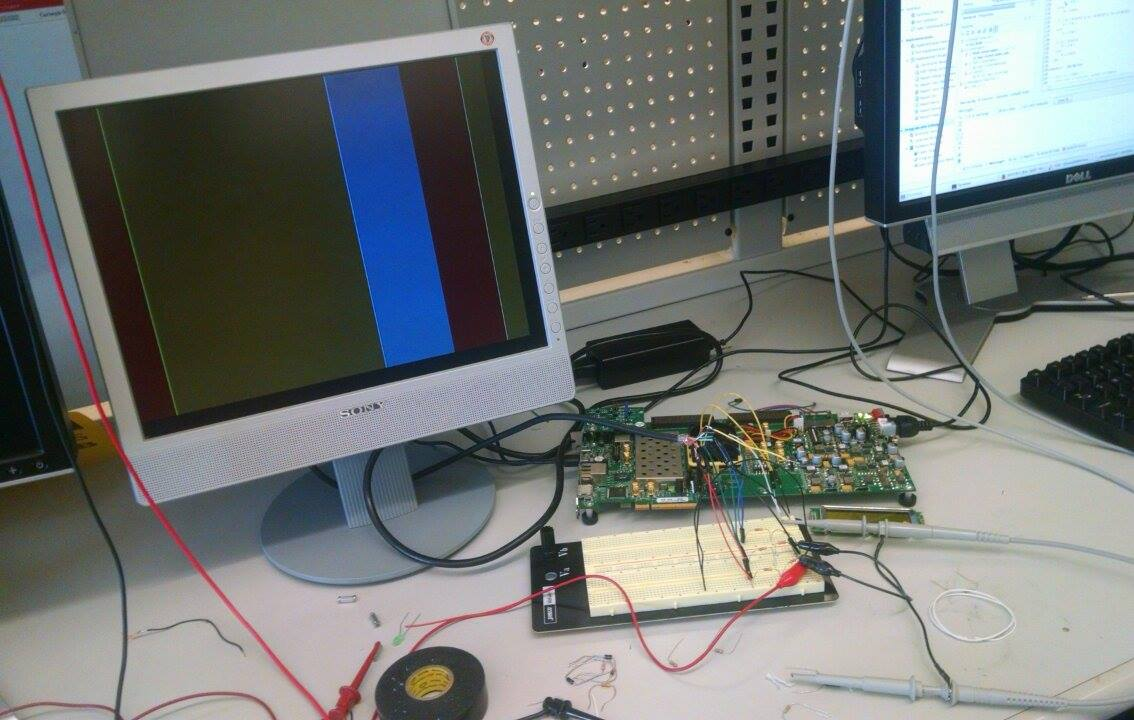
\includegraphics[width=4in]{Diagrams/VGA.jpg}\\
    \textit{A totally stable VGA system}
  \end{center}
}

\frame{
  \frametitle{Progress}
  \begin{itemize}
    \item What does not work:
      \begin{itemize}
        \item PS/2
          \begin{itemize}
            \item Not yet implemented
            \item No PS/2 port; less of a problem than VGA: not analog
          \end{itemize}
        \item Amber Core Modifications
          \begin{itemize}
            \item OOO - Hard, but design is pretty solid
            \item Superscalar - Also hard, design is getting close
            \item MorphCore - flush the cache, flush the pipeline, switch modes!
          \end{itemize}
      \end{itemize}
  \end{itemize}
}

\section{Questions}

\end{document}